% Drawing 67/03-3 -- folder 67, batch 03, archive page 56 (PDF page 57).
% Transcription: dans la marge gauche, à hauteur du passage encadré : un arc descendant qui fait un coin en un point marqué (le point $x$), un ovale en tirets autour de ce point, avec une croix à l'intérieur, et à droite du coin une région hachurée entre une corde et un arc.
% Kind: arc with a corner at a marked point, dashed neighbourhood, hatched region. Method 2 (schematic redraw from the facsimile). Status: partial.
% Notes: As on the page: the arc comes down from the upper right, turns back to a heavy point at the tip of a wedge (the point x of the lemma), and goes on downwards; round the point a dashed oval, with a small cross inside it at the lower left; right of the wedge a region bounded by a straight stroke and an arc, hatched obliquely. Arc, wedge and the straight stroke are drawn through the same computed points. Still differs: the hatching is five strokes on the page, set by the pattern here; the dashed oval is an ellipse fitted to his broken outline. The transcription's note says « un point $x$ sur un arc, un voisinage en pointillé, une rive hachurée »: agreed, save that the letter x is not written by the sketch (a cross stands inside the oval). Redrawn 2026-11-12 (issue 128): to check again.
% Coordinates: 1 unit = 1 mm = 1/100 of the crop width (bbox in page fractions: [0.11, 0.23, 0.27, 0.31]).
% Redrawn by Claude (claude-fable-5-2), issue #128, 2026-11-12; not checked by a human; not compiled (no TeX in the session).
% Rights: reproduces part of the work -- behind RENDER_TRANSCRIPTS, never published by itself.
\documentclass[tikz,border=3pt]{standalone}
\usepackage{amsmath,amssymb}
\usetikzlibrary{patterns,arrows.meta}
\tikzset{pencil/.style={black!45}, struck/.style={black!35}, mpt/.style={circle,draw,inner sep=1.3pt}, pt/.style={circle,fill,inner sep=0.9pt}, opt/.style={circle,draw,fill=white,inner sep=1.1pt}}
\begin{document}
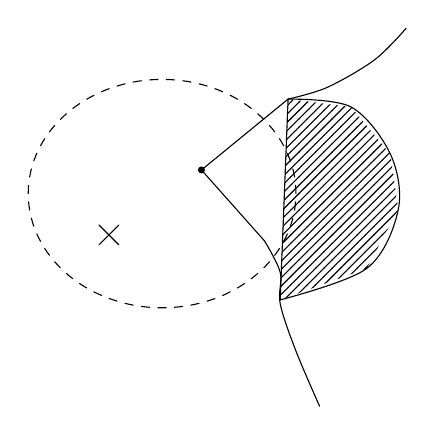
\begin{tikzpicture}[x=1mm,y=1mm,line cap=round,line join=round,font=\scriptsize]
\draw[dashed] (57,-41) ellipse[x radius=17, y radius=14.5];
\draw plot[smooth, tension=0.55] coordinates {(88,-20) (84,-24) (78,-27.5) (73,-29)};
\draw (73,-29) -- (62,-38) -- (70,-47);
\draw plot[smooth, tension=0.55] coordinates {(70,-47) (72,-51) (72,-55) (74,-61) (77,-68)};
\node[pt] at (62,-38) {};
\draw (73,-29) -- (72,-54.5);
\draw plot[smooth, tension=0.55] coordinates {(73,-29) (81,-30) (86,-36) (87,-43) (83,-50.5) (72,-54.5)};
\fill[pattern=north east lines] (73,-29) -- (81,-30) -- (86,-36) -- (87,-43) -- (83,-50.5) -- (72,-54.5) -- cycle;
\draw (49,-45) -- (51.5,-47.5);
\draw (51.5,-45) -- (49,-47.5);
\end{tikzpicture}
\end{document}
